\documentclass[12pt, a4paper, twoside]{article} %twoside is for fancyhdr





%--------------------------------------------------------------------------%
%--------------------------------------------------------------------------%
% ------------------------------  PACKAGES --------------------------------%
%--------------------------------------------------------------------------%
%--------------------------------------------------------------------------%






% ----------------------  GENERIC DOCUMENT SETTINGS -----------------------%
%--------------------------------------------------------------------------%
\usepackage{geometry}  
	\geometry{top = 3.5cm, bottom = 3cm, left = 2cm, right = 2cm, headsep = 1.4cm, footskip = 1.5cm}
\usepackage[skip = 7pt, indent = 0pt]{parskip} % paragraph settings
\usepackage{titlesec}%first parameter to set specific indentation to each section
					 %second and third paarmeters to set before and after spacing
					 % in section, subsection y subsubsection
    \titlespacing\section{0pt}{0.6cm}{0.6cm}
    \titlespacing\subsection{0pt}{0.5cm}{0.5cm}
    \titlespacing\subsubsection{0pt}{12pt plus 4pt minus 2pt}{5pt plus 2pt minus 2pt}
\usepackage{microtype} %improves the justification, and therefore the visualization of the text
\usepackage{times} %font family to times new roman
%%\usepackage{fontspec}%font-family
	%%\setmainfont{Verdana} %FALSE POSITIVE ERROR
	
\usepackage{hyperref} %links: internal & external
\hypersetup{ %for all kinds of links. It has more parameters but
	% we are just going to use the most basic ones
    colorlinks = true,
    linkcolor = blue, % internal links
    urlcolor = orange, % external links
    filecolor = green % link to your files
} % ------------- USE \hyperlink for internal link and \href for external ------------------%

\usepackage{fancyhdr} % To create custom headers and footnotes
%\fancypagestyle{plain}{ % este es un tipo de header y footer. Lo he llamado plain. 
%	\fancyhead{} % clear header
%	
%	\fancyhead[L]{\nouppercase\leftmark}
%	\fancyhead[RE]{\text{Trabajo Fin de Grado}}
%	\fancyhead[RO]{\text{Análisis de Series Temporales}}
%	\fancyfoot{} % clear footnote
%	\fancyfoot[RE]{\text{U-tad 2023-2024}} 
%	\fancyfoot[RO]{\text{MAIS}}
%	\fancyfoot[C]{\thepage}
%	\fancyfoot[L]{\text{Javier Coque}}
%	\renewcommand{\footrulewidth}{0.4pt}% default is 0pt
%}

%--------------------- NOTA IMPORTANTE -------------------------%
%---------------------------------------------------------------%
%Me acabo de crear arriba un estilo que se llama plain;  le podría haber llamado bocata. Para aplicar dicho header, basta con poner \pagestyle{plain} al principio del documento para que se aplique.


%El comando \leftmark sirve para asignar como texto el título de la sección. El caso es que solo funciona para secciones numeradas. Para que también funcione en secciones no numeradas deberemos usar el siguiente comando: \markboth{nombre_seccio_no_numerada}{nombre_seccion_no_numerada}. El primer parámetro indica lo que poner en páginas pares y el segundo en impares, así que se puede modificar a gusto propio.

%En caso de querer usar un estilo propio en alguna de las secciones, se puede hacer con \thispagestyle{fancy} y luego aplicar las customizaciones que quieras como pueden ser \fancyfoot[L]{\text{nuevo_foot_text}}. Al acabar, vuelve a poner el comnado \pagestyle{plain} para volver al otro estilo.

%Otra cosa que se puede hacer es crear  varios estilos de fancyhdr. Al igual que me he creado el estilo plain, me puedo cerar otros. 

%Lo que acabo de explicar está en mi TFG de matemáticas hecho.
%--------------------------------------------------------------------------%
%--------------------------------------------------------------------------%





% -----------------------  FOR MORE SUBSECTIONS ---------------------------%
%--------------------------------------------------------------------------%
% Define a custom heading for the fourth level
%%\newcommand{\subsubsubsection}[1]{\paragraph{#1}\mbox{}\\} %now I do have subsubsubsubsection
%%\setcounter{secnumdepth}{4} % how many sectioning levels to assign numbers to
%%\setcounter{tocdepth}{4} % Enable numbering for up to the fourth level
%--------------------------------------------------------------------------%
%--------------------------------------------------------------------------%





% --------------------==------  FOR MATH STUFF ----------------------------%
%--------------------------------------------------------------------------%
%%\usepackage{amsmath,amsfonts,amsthm, amssymb} % Para poder usar \mathbb
	%%\renewcommand{\qed}{\hfill\blacksquare} %blacksquare for demonstrations
%%\numberwithin{equation}{subsection} %this numbers the equatino along with the subsections
%%\usepackage{cancel} %to cancel numbers in  equations
%%\usepackage{mathtools} %to annotate brackets in equations
%--------------------------------------------------------------------------%
%--------------------------------------------------------------------------%





% ----------------------  FIGURES , TABLES & TIKZ  ------------------------%
%--------------------------------------------------------------------------%
\usepackage{graphicx}
    \graphicspath{ {./imgs/} }
%%\counterwithin{figure}{section}%figure number along with the section
%%\usepackage{subfigure} % for subfigures
%%\usepackage{wrapfig} % to wrap a figure among text
%%\usepackage{caption} % caption management in figures and tables
	%%\captionsetup[figure]{name=Figura}%Changes the default name Figure to Figura in figures
\usepackage{float} % for H command in figures and tables
%%\usepackage{listings} % para poder hacer uso de "listings" propios (p.ej. códigos)
%%	\lstset{
%%		language=Python,
%%		basicstyle=\ttfamily\small,
%%		keywordstyle=\bfseries\color{blue},
%%		stringstyle=\color{orange!70!black},
%%		commentstyle=\color{green!70!black},
%%		showstringspaces=false,
%%		frame=single,
%%		breaklines=true,
%%		captionpos=b
%%	}
\usepackage{longtable} % Para tablas muy largas
\usepackage{array} % for table's setting such as spacing within cells and 
				   % the border width
\renewcommand{\tablename}{Tabla} % %Changes the default name Table to Tabla in tables
%\newcolumntype{s}{>{\columncolor{blue!15}} c} %command for a specific type of column.
\renewcommand{\arraystretch}{3} % top and bottom spacing inside table's cells				   	
\usepackage{multirow} % Para agrupar varias filas en las tablas


\usepackage{tikz}
    \usetikzlibrary{shapes,arrows, positioning}
    \usetikzlibrary{patterns}
\usepackage{pgfplots}
    \usepgfplotslibrary{fillbetween}% color tikz's images
    \pgfplotsset{compat=1.17} %this can be change to compat = newest
%--------------------------------------------------------------------------%
%--------------------------------------------------------------------------%





% ---------------  TCOLORBOXES, COLORS AND OTHER DECORATIVES  -------------%
%--------------------------------------------------------------------------%
\usepackage{xcolor}  % color package to create colors. Additional table features added to xcolor package
%ATTENTION:NO SPACING IN COLOR RGB VALUES
	% ------------ RGB style -----------%
	\definecolor{redos}{RGB}{255,46,46}
	\definecolor{redcl}{RGB}{255,200,200}
	% ------------ HTML CODE style -----------%
	\definecolor{azulos}{HTML}{4291FD}
	\definecolor{azulcl}{HTML}{E8F3FF}
	
\usepackage[most]{tcolorbox} % package to create color boxes  like the note box

\newtcolorbox{atencion}{
	enhanced,
	breakable,
	fonttitle=\sffamily\bfseries,
	colbacktitle=redcl,
	coltitle=redos,
	title= Atencion:,
	colbacktitle=redcl,
	title code={
		\path[draw=redos,solid,line width=0.75mm]
		([xshift=0mm]title.south west) -- ([xshift=0mm]title.south east);
	},
	boxrule=0pt,frame hidden,
	borderline west={3pt}{0pt}{redos},
	colback=redcl,
}

\newtcolorbox{demo}[1]{
	enhanced,
	breakable,
	fonttitle=\sffamily\bfseries,
	colbacktitle=azulos,
	coltitle=azulos,
	title= #1,
	colbacktitle=azulcl,
	boxrule=0pt,frame hidden,
	borderline west={3pt}{0pt}{azulos},
	colback=azulcl,
	top = 10pt, %body margin
	before title={\vspace*{5pt}}, %title margin
	bottom = 8pt
}

\newtcolorbox{teorema}[1]{
	enhanced,
	breakable,
	fonttitle=\sffamily\bfseries,
	colbacktitle=azulcl,
	coltitle=azulos,
	title= #1,
	colbacktitle=azulcl,
	title code={
		\path[draw=azulos,solid,line width=0.75mm]
		([xshift=5mm]title.south west) -- ([xshift=0mm]title.south east);
	},
	boxrule=0pt,frame hidden,
	borderline west={3pt}{0pt}{azulos},
	colback=azulcl,
}

\newtcolorbox{ejemplo}[1]{
	enhanced,
	breakable,
	fonttitle=\sffamily\bfseries,
	%colbacktitle=azulos,
	coltitle=azulos,
	title=#1,
	%colbacktitle=azulcl,
	boxrule=0pt,frame hidden,
	borderline west={3pt}{0pt}{azulos},
	colback=azulcl,
}
\newtcolorbox{ejemplo2}[1]{
	enhanced,
	breakable,
	fonttitle=\sffamily\bfseries,
	colbacktitle=azulcl,
	coltitle=azulos,
	title= #1,
	colbacktitle=azulcl,
	title code={
		\path[draw=azulos,solid,line width=0.75mm]
		([xshift=0mm]title.south west) -- ([xshift=0mm]title.south east);
	},
	boxrule=0pt,frame hidden,
	borderline west={3pt}{0pt}{azulos},
	colback=azulcl,
}


\newtcolorbox{nota}{
	enhanced,
	breakable,
	fonttitle=\sffamily\bfseries,
	%colbacktitle=azulos,
	coltitle=azulos,
	title=Nota,
	colbacktitle=azulcl,
	boxrule=0pt,frame hidden,
	%borderline west={3pt}{0pt}{azulos},
	colback=white,
}

%\newtcolorbox{mathbox}{
%	colback = white,
%	colframe = azulos,
%}
%
%
%\newenvironment{matheq}{%
%	\begin{center}%
%		\begin{mathbox}%
%		}{%
%		\end{mathbox}%
%	\end{center}%
%}
%
%\newenvironment{matheq2}{%
%	\begin{center}%
%		\tcbox[colback = azulcl, colframe = azulos]%
%	}{%
%	\end{center}%
%}
%--------------------------------------------------------------------------%
%--------------------------------------------------------------------------%




% --------------------------  MISCELLANEOUS  ------------------------------%
%--------------------------------------------------------------------------%
\usepackage{comment} %to comment big sections with \begin{comment}...\end{comment}
\usepackage{enumitem} %for lists
\usepackage{url} %to place url with te command \url{https://...}
\usepackage{environ}% to create new environments

%--------------------------------------------------------------------------%
%--------------------------------------------------------------------------%




% --------------------------  REFERENCES  --------------------------------%
%-------------------------------------------------------------------------%
\usepackage[backend = biber, style = numeric]{biblatex} %change styple to apa if necessary
%\DeclareLanguageMapping{spanish}{spanish-apa}
\addbibresource{biblio.bib} % Fichero donde se incluyen las referencias
%---------------------------------------------------------------------------------------%
%---------------------------------------------------------------------------------------%








%---------------------------------------------------------------------------------------%
%---------------------------------------------------------------------------------------%
% -------------------------  NEW COMMANDS & NEW ENVIRONMENTS ---------------------------%
%---------------------------------------------------------------------------------------%
%---------------------------------------------------------------------------------------%




% ---------------------  GENERIC DOCUMENT SETTINGS ------------------------%
%--------------------------------------------------------------------------%
\renewcommand{\baselinestretch}{1.4}% Espaciado entre líneas
%\usepackage{setspace} %espaciado entre lineas de manera no tan precisa 
	%\onehalfspacin
\newcommand{\B}[1]{\textbf{#1}}
\newcommand{\slas}{$\backslash$}
\newcommand{\ti}{\emph} %it stands for text italic. The command \it is already taken.
\newcommand{\ul}{\underline}
\newcommand{\fn}{\footnote}
\newcommand{\fnm}{\footnotemark}
\newcommand{\fnt}{\footnotetext}
    \setlength{\footnotesep}{\baselineskip}%increase spacing between footnotes
% CHANGE THE DEFAULT NAME OF TOC AND LIST OF FIGURES/TABLES AT THE BEGINNING.
% i.e. when using \tableofcontents, \listoffigures, \listoftables in \begin{document}
%\renewcommand{\contentsname}{Tabla de contenidos}%cambiar titulo de \listofcontents (contents por defecto)
%\renewcommand{\listfigurename}{Lista de Figuras}
%\renewcommand{\listtablename}{Lista de Tablas}
%--------------------------------------------------------------------------%
%--------------------------------------------------------------------------%




	
% -------------------------------  MATH  ----------------------------------%
%--------------------------------------------------------------------------%
%This is to display inline math symbols as if they were block symbols. Shorten commands intead of
%using displaystyle... .
\newcommand{\Int}[2]{\displaystyle \int_{#1}^{#2}}
\newcommand{\Sum}[2]{\displaystyle \sum_{#1}^{#2}}
\newcommand{\Lim}[1]{\displaystyle \lim_{#1}}
\newcommand{\Frac}[2]{\displaystyle \frac{#1}{#2}}

%Make shorter the command to write the N of Naturals, Z of Integer,  R of Reals, Q of rational & C of complex
\newcommand{\N}{\mathbb{N}}
\newcommand{\Z}{\mathbb{Z}}
\newcommand{\Q}{\mathbb{Q}}
\newcommand{\R}{\mathbb{R}}
\newcommand{\C}{\mathbb{C}}

%to be able to write the text Var, Cov and Corr in math equations
\newcommand{\Var}{\mathrm{Var}}
\newcommand{\Cov}{\mathrm{Cov}}
\newcommand{\Corr}{\mathrm{Corr}}
%--------------------------------------------------------------------------%
%--------------------------------------------------------------------------%




% --------------------------  MISCELLANEOUS  ------------------------------%
%--------------------------------------------------------------------------%
\newcommand{\Code}[1]{\fcolorbox{code}{code}{\slas #1}} %to write words meaning a command or code
	\definecolor{code}{RGB}{228, 229, 231}
	
% Para que el índice no sea clickable
%\makeatletter
%\let\Hy@linktoc\Hy@linktoc@none
%\makeatother

% To avoid word splitting between lines. Example: (first line) misce- (seccond line) llaneous.
%\pretolerance=10000
%--------------------------------------------------------------------------%
%--------------------------------------------------------------------------%




\title{Informe sprint 2\\
\large Proyectos IV: Equipo BI\\
\large Proyecto: ERP}
\author{
  \small{Juan Carlos Ávila}\fn{juan.avila@live.u-tad.com}
  \and
  \small{Javier Coque}\fn{javier.coque@live-u.tad.com}
  \and
  \small{Alejandro García}\fn{alejandro.gallego@live.u-tad.com}
  \and
  \small{Chantal López}\fn{chantal.lopez@live.u-tad.com}
}
\date{9, marzo 2024}

\begin{document}
\maketitle


\pagenumbering{arabic}
\pagestyle{plain} % setting our default header and footer that we set with
% ÍNDICE DE CONTENIDOS
\setcounter{page}{1}

\section{Resumen Sprint 2}
Este \ul{Sprint 2} constaba de tres \B{historias} principales: 
\begin{itemize}
    \item \B{Historia 1}: Como comprador quiero poder realizar una compra mediante un botón de compra en Odoo.
    \item  \B{Historia 2}: 
    \begin{itemize}
        \item a) \hspace{5pt} Como \B{vendedor} me gustaría poder cancelar un pedido.
        \item b) \hspace{5pt} Como \B{comprador} me gustaría poder cancelar un pedido.
    \end{itemize}
    \item \B{Historia 3}: Como usuario me gustaría poder visualizar las ventas de mis compras y pedidos.
\end{itemize}

\subsection{Historia 1: Yo como comprador quiero poder realizar una compra mediante un botón de compra en Odoo}
Esta historia se ha dividido en 8 tares de las cuales se han hecho 4 y no ha dado tiempo a hacer 2.

\subsubsection{Hechas}
Las dos tareas que se han realizado durante este Sprint 2 son las de:
\begin{itemize}
    \item \B{Generar un botón de compra}: El objetivo de esta tarea era el de poder crear un botón de compra en el módulo de \texttt{Compras} para permitir al usuario poder realizar esta acción en dicho módulo.
    
    \item \B{Crear fecha de entrega}: Otra de las cosas que se ha conseguido hacer este Sprint 2 es la tarea de, una vez realizada una compra. crear un campo \B{Fecha de entrega} en la que se indique al cliente que acaba de realizar la compra, la fecha esperada de entrega. 

\end{itemize}
\begin{ejemplo}{Nota}
    Se espera para \ul{el próximo Sprint} implementar alguna lógica a esta fecha de entrega. Algunas ideas que se barajan por el momento son las de basar esta fecha de entrega en base al precio de la compra o del los productos en stock. No está decidido aún.
\end{ejemplo}
\begin{itemize}
    \item \B{Desencolar una petición de producto.}
    
    \item \B{Encolar una petición de confirmación de pedido.}
    
    \item \B{Desencolar la confirmar del pedido.} 
    
    \item \B{Encolar una petición de producto.}
\end{itemize}

Como se comentó en la auditoría del \ul{Sprint 1}, se ha decidido utilizar como sistema de mensajería Kafka (en vez de RabbitMQ, que era la otra opción). 

El objetivo de estas tareas es que, al pulsar un botón en Odoo---realizar un pedido por parte del cliente o confirmar el pedido por parte del vendedor respectivamente---, esta petición se encolase en un \B{Topic} de Kafka por parte del \ti{Producer}, para que posteriormente pudiera ser desencolado por el \ti{Consumer}.

Un problema que se ha encontrado a la hora de realizar estas tareas, es que, en un primer momento, no se conseguía establecer una comunicación entre los contenedores de Odoo y de Kafka dentro de la misma \ti{network} en Docker.

Finalmente, después de investigar, se encontró el problema y se pudo solucionar. Esta solución pasó por añadir una regla de \ti{Docker-Compose} para que habilitara el puerto local. 

Se  deja una gráfica que muestra visualmente la arquitectura diseñada de Docker que hay por detrás para habilitar encolar y desencolar en Kafka. Véase figura \ref{subred1}.


\begin{figure}[H]
    \centering
    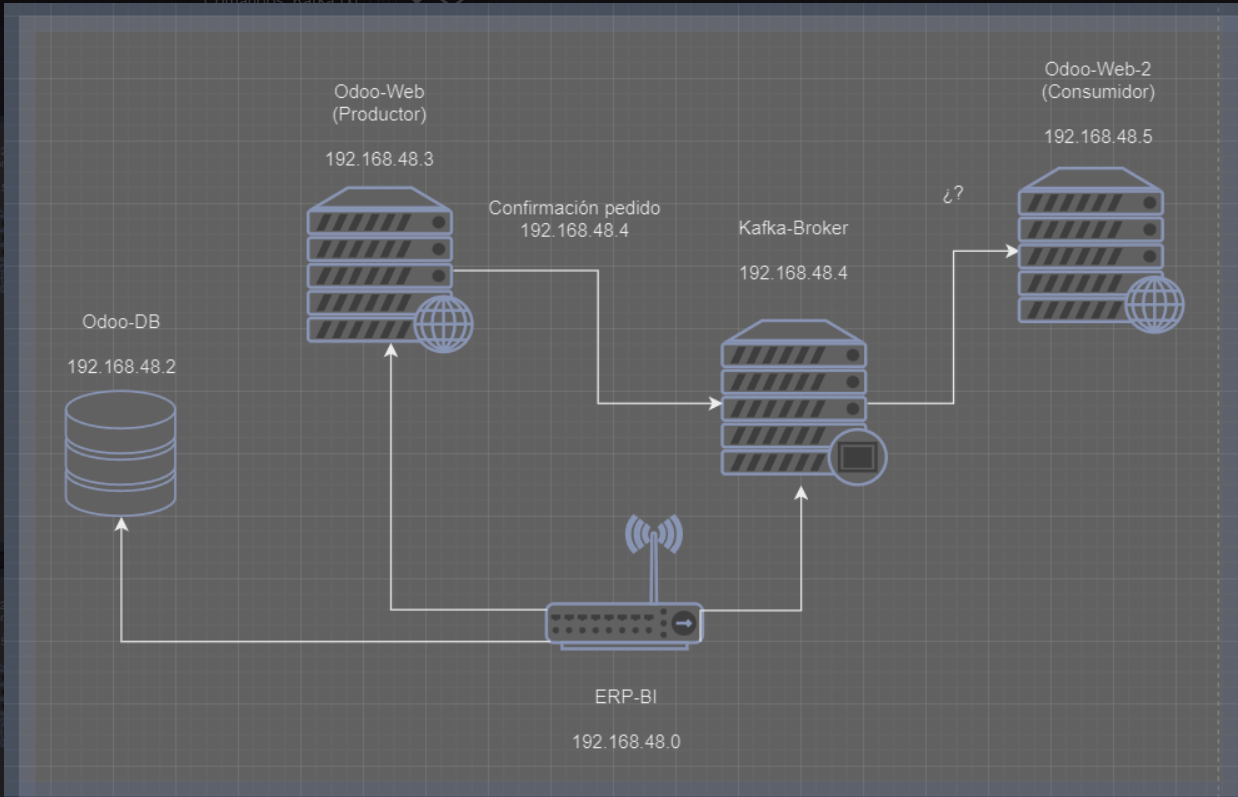
\includegraphics[width = 0.8\textwidth]{aa_imgs/img_arq_1}
    \caption{Subred Docker.}
    \label{subred1}
\end{figure}

\begin{ejemplo}{Nota}
Se deja al final de este documento cómo hay que modificar esta red en los siguientes Sprints (figura \ref{subred2}).
\end{ejemplo}


\subsubsection{No ha dado tiempo}
De esta historia, han quedado dos tareas por hacer. Estas tareas son:
\begin{itemize}
    \item  \B{Actualizar el estado del pedido}: Esta tarea tenía como objetivo poder mostrar al cliente el estado de su pedido. En principio, se había pensado que este estado podía ser: 
    \begin{enumerate}
        \item Pedido pendiente de confirmar.
        \item Pedido confirmado.
        \item Pedido Enviado.
        \item En espera de recogida.
        \item Entregado
    \end{enumerate}
    \item  \B{Enviar un mensaje de confirmación al vendedor}
    
\end{itemize}

\subsection{Historia 2$_{a}$: Como comprador me gustaría cancelar un pedido}

Esta historia se ha dividido en 4 tareas: 3 que he han hecho y 1 que no ha dado tiempo.

\subsubsection{Hechas}
Entre las tareas que se han hecho, se encuentran:
\begin{itemize}
    \item  \B{Botón desde el módulo de Compras a Pedidos}: Crear un botón para desde la sección de \texttt{Compras} poder ser redirigidos---nosotros como clientes--- a la sección de \texttt{Ventas}. Esta es una tarea previa y necesaria para la siguiente.
    
    \item \B{Botón para cancelar un pedido}: Crear un botón desde la sección de \texttt{Ventas} para poder cancelar un pedido realizado.
\end{itemize}

\subsubsection{No ha dado tiempo}
De esta historia, ha habido únicamente 1 tarea que no ha dado tiempo a completar. Esta tarea se la de:
\begin{itemize}
    \item  \B{Cancelación de pedido en un rango de tiempo}: La idea que habíamos tenido es la de que el comprado pudiera cancelar un pedido en un rango de tiempo determinado, e.g. en las primeras 24h. Para \ul{el próximo Sprint} se baraja la idea de cambiar la condición de tiempo por la del estado de producto, e.g. si el producto tiene un estado de \ti{enviado} o \ti{en espera de recogida}, entonces que no se pueda cancelar el producto.
\end{itemize}

\subsection{Historia 2$_{b}$: Como vendedor me gustaría cancelar un pedido}

Las tareas de la historia anterior son las mismas que esta con una pequeña modificación, pues ahora es desde el punto de vista del vendedor: la cancelación de pedido la realiza el vendedor con un criterio no establecido. En palabras más coloquiales, el vendedor puede cancelar un pedido \ti{si le da la gana}. 

\subsubsection{No ha dado tiempo}

\begin{itemize}
    \item  \B{Cancelación de pedido por parte del vendedor}
\end{itemize}

\subsection{Historia 3: Como vendedor me gustaría poder visualizar las ventas de mis pedidos}
Para esta historia, nuestro equipo se había comprometido a crear un módulo para poder mostrar un Dashboard BI. El objetivo era el de mostrar, al menos, un par de gráficas muy sencillas. En el \ul{próximo Sprint} se investigará más a fondo cómo añadir más gráficas y perfeccionar las ya existentes.

\subsubsection{Hechas}
\begin{itemize}
    \item \B{Dashboard de compras}: El objetivo de esta tarea era que el usuario pudiera ver distintos gráficas en las que se pudiera visualizar información acerca de sus \B{compras}.
    \item \B{Dashboard de ventas}: El objetivo de esta tarea era que el usuario pudiera ver distintos gráficas en las que se pudiera visualizar información acerca de sus \B{ventas}.
\end{itemize}

Algunos de los problemas que se han encontrado en ese apartado son los siguientes:
\begin{itemize}
    \item Crear una vista que pueda contener más de una gráfica.
    \item Generar una gráfica específica. Es decir, en vez de mostrar una única gráfica de un tipo (barras, líneas, pieChart), se muestra la de barras por defecto, dejando al usuario libertad para elegir cualquier otro tipo de gráfica
\end{itemize}
Para el primer problema, lo que se ha 

Para el primer problema, la solución que se ha pensado---y llevado a cabo--- es la de generar dos submenús (una para compra y otro para venta) y dentro de estos submenús crear una página distinta para cada gráfica. Indicando al usuario, por supuesto, qué página (vista) muestra qué gráfica.

El segundo problema, en realidad, se puede ver como una ventaja, pues el usuario tiene más libertad acerca de en qué grafica(s) quiere visualizar unos datos determinados.
\section{Ideas para siguiente Sprint}

\begin{itemize}
    \item Añadir una confirmación al botón de confirmar pedido.
    \item IP estática---i.e. la misma para todos--- en el \ti{Docker-Compose} para la red de Docker. De esta manera, la conexión entre los contenedor dentro de la red está homogeneizada.
    \item Computar el campo de Fecha de entrega en base a una lógica.
    \item Encriptar la cola de mensajería de Kafka.
    \item Terminar de desencolar los pedidos en Kafka. En otras palabras, se tiene que ver cómo convertir el Odoo\_web2 en un \ti{Kafka Consumer}.
    \item Establecer una autenticación única para que el Productor y Consumidor de Kafka sean los únicos habilitados para leer los mensajes de sus respectivos Tópicos asignados.
    \item Añadir gráficas más representativas al módulo de Gráficas.
\end{itemize}

Como se comentó con anterioridad, se deja una imagen de la subred de Docker que se espera tener en el próximo Sprint.
\begin{figure}[H]
    \centering
    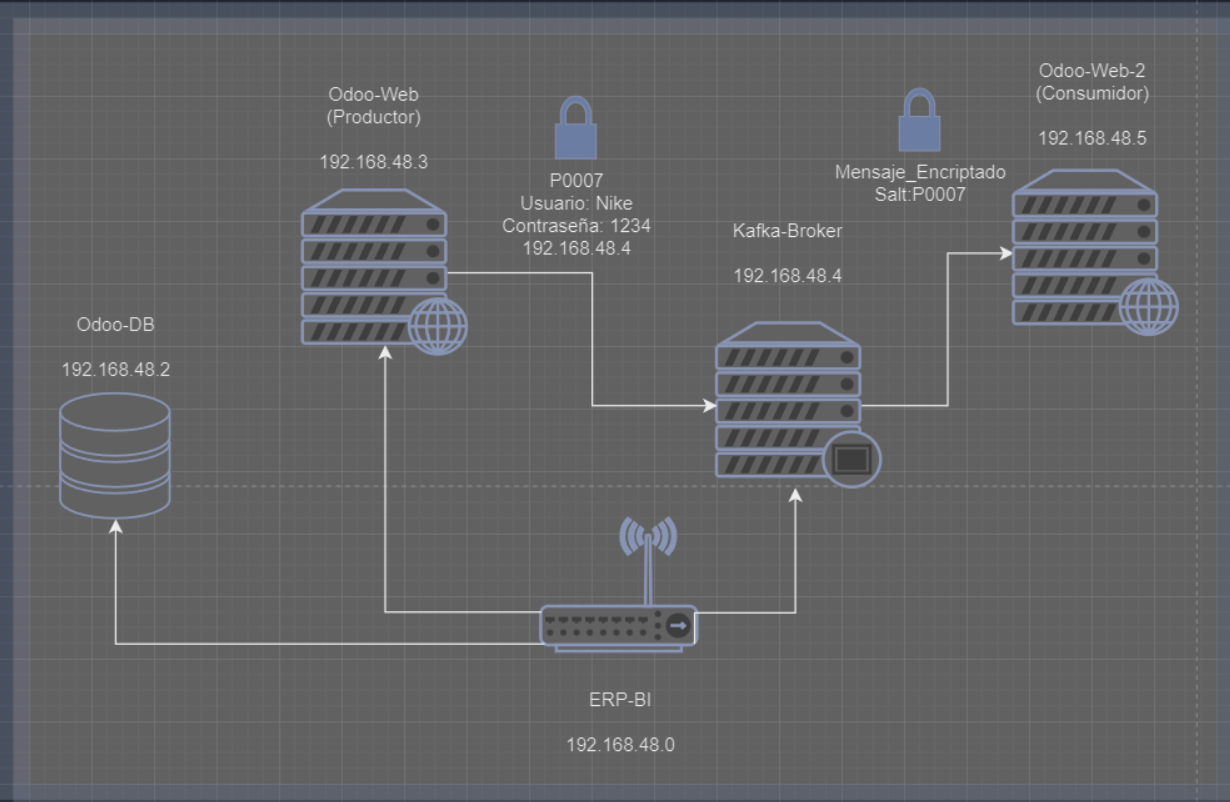
\includegraphics[width = 0.8\textwidth]{aa_imgs/img_arq_2}
    \caption{Subred Docker}
    \label{subred2}
\end{figure}

\end{document}

